\documentclass[a4paper]{beamer}
\usepackage[italian]{babel}
\usepackage[utf8]{inputenc}

\usepackage{graphicx}
\usepackage{wrapfig}
\usepackage{eurosym}
\useoutertheme{weeeopentheme}

\title{WEEE Open}
\subtitle{Workshop - Architettura di un calcolatore}
\author{Giorgio Pais}
\institute{Politecnico di Torino}
\date{a.a. 2017/2018}

\definecolor{bluew}{HTML}{2a66a2}
\definecolor{dbluew}{HTML}{25598e}

\setbeamercolor{title}{fg=dbluew}
\setbeamercolor{alerted text}{fg=bluew}
\setbeamercolor{example text}{fg=bluew}
\setbeamercolor{frametitle}{fg=white, bg=bluew}

\begin{document}

	\frame{\titlepage}
	
	\begin{frame}
		\frametitle{\begin{LARGE}Indice\end{LARGE}}
		\tableofcontents
	\end{frame}

	\section{Scheda Madre}
	\begin{frame}
	\frametitle{\begin{LARGE}
			Scheda Madre - Introduzione
		\end{LARGE}}
		\begin{Large}
			\textbf{Vedremo}\par
		\end{Large}
		\begin{itemize}
			\item[-] Standard utilizzati
			\item[-] Architettura e chipset
			\item[-] Componenti a rischio rottura
			\item[-] Accenni al debug
		\end{itemize}
	\end{frame}

	\begin{frame}
		\frametitle{\begin{LARGE}Scheda Madre\end{LARGE}}
		\begin{Large}
			{Standard, viteria, attrezzi da utilizzare e principio di funzionamento.}
		\end{Large}\par
		\vspace{0.6cm}
		\begin{wrapfigure}{1}{5cm}
			\vspace{-0.3cm}
			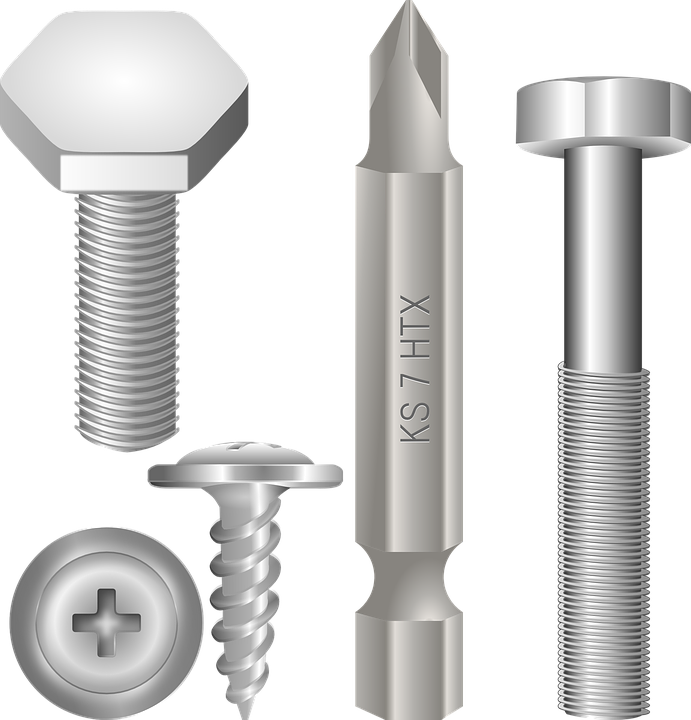
\includegraphics[width=4.5cm]{images/viti}
			\hspace{0.5cm}
		\end{wrapfigure}
		\hspace{0.4cm}\begin{Large}
			\hspace{-0.7cm}	\textbf{Viteria}:
		\end{Large}
		\begin{itemize}
			\item[-] \#6-32 UNC 
			\item[-] M3
			\item[-] Distanziali esagonali
			\item[-] \#4-40 UNC
			\item[-] Spessori/cable management
			\item[-] Alimentatore, dissipatore e altre viti
		\end{itemize}
	\end{frame}

	\begin{frame}
		\frametitle{\begin{LARGE}Scheda Madre\end{LARGE}}
		\begin{wrapfigure}{1}{6cm}
		\vspace{0.4cm}
		\hspace{-2cm}
		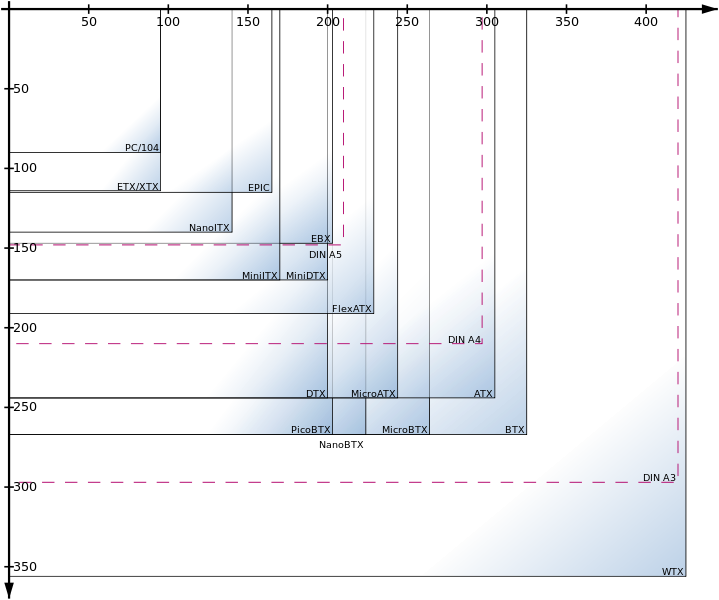
\includegraphics[width=7cm]{images/formsfac}
		\end{wrapfigure}
		\begin{Large}
			\vspace{-3cm}
			\textbf{Fattori di forma}:
		\end{Large}\\
	\vspace{0.1cm}
		\hspace{0.2cm}\text{    - ATX} \\
		\hspace{0.2cm}\text{  - Altri}
	\end{frame}
	
	\begin{frame}
	\frametitle{\begin{LARGE}Scheda Madre\end{LARGE}}
	\begin{wrapfigure}{1}{4cm}
		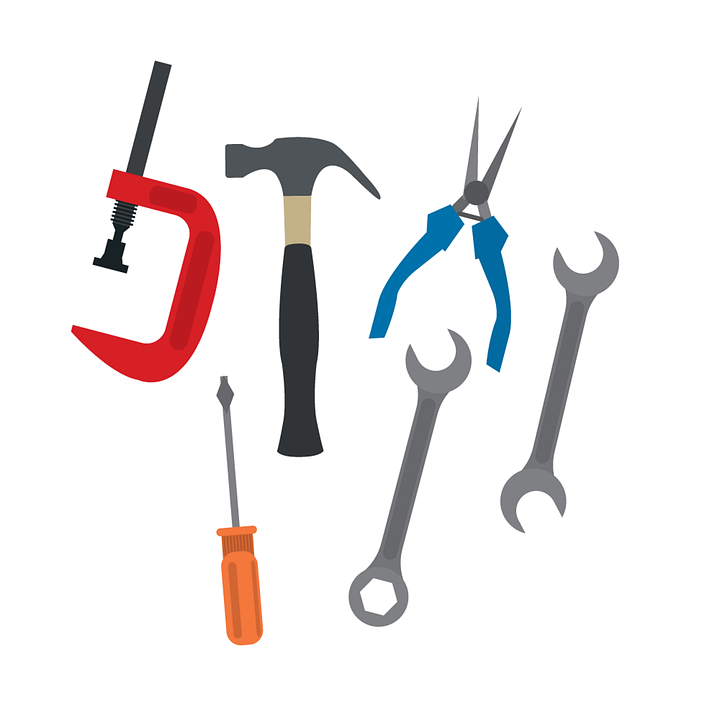
\includegraphics[width=4cm]{images/att}
	\end{wrapfigure}
	\hspace{-0.1cm}
	\begin{Large}
		\vspace{-0.5cm}\textbf{Attrezzi}:
	\end{Large}
	\vspace{0.6cm}
	\begin{itemize}
		\item[-] Cacciaviti
		\item[-] Pinze e pinzette
		\item[-] Jumper
		\item[-] Fascette
		\item[-] Multimetro, oscilloscopio e debugger
		\item[-] Saldatore e stazione ad aria calda
		\item[-] Altri vari attrezzi/accessori
	\end{itemize}
	\end{frame}

	\begin{frame}
		\frametitle{\begin{LARGE}Scheda Madre\end{LARGE}}
		\begin{wrapfigure}{1}{6.5cm}
			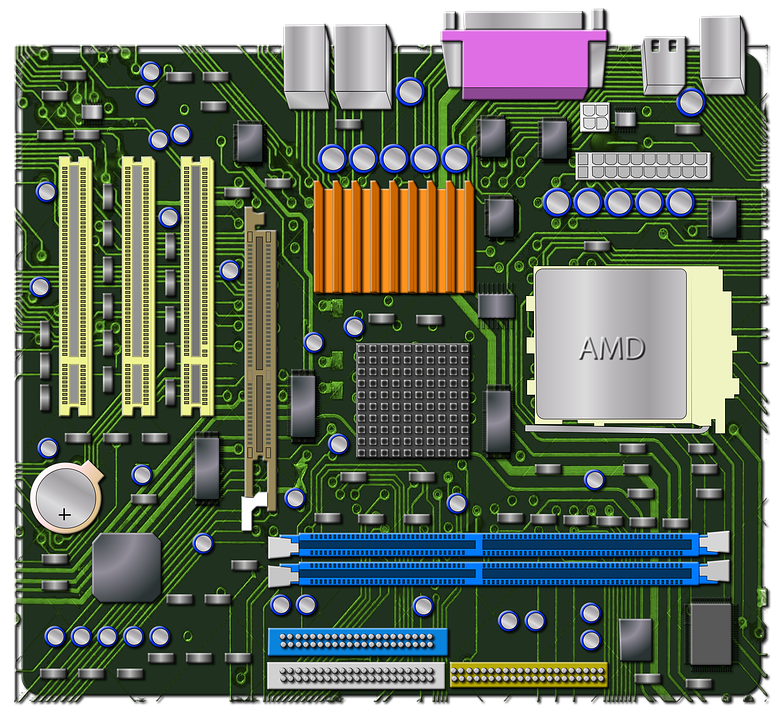
\includegraphics[width=6cm]{images/mtb}
		\end{wrapfigure}
		\hspace{1cm}\begin{Large}
			\hspace{-1cm}\textbf{Funzionamento}:
		\end{Large}\par
		\begin{itemize}
			\item[-] Bus e interconnessioni
			\item[-] Clock
			\item[-] Periferiche
			\item[-] Porte e connettori
			\item[-] Socket
			\item[-] Chipset (Northbridge + Southbridge)
			\item[-] BIOS 
		\end{itemize}
	\end{frame}
	
		\begin{frame}
	\frametitle{\begin{LARGE}Bus e interconnessioni\end{LARGE}}
	\begin{Large}{
		\begin{LARGE}
			\textbf{Il bus}.
		\end{LARGE}\\ Si tratta di un collegamento dati generico punto-multipunto, progettato per permettere di collegare alla scheda madre delle altre schede di espansione alloggiate su connettori, che ne estendono le capacità.}
	\end{Large}
\end{frame}

		\begin{frame}
	\frametitle{\begin{LARGE}Periferiche\end{LARGE}}
	\begin{Large}{
			\begin{LARGE}
				\textbf{Le periferiche}.
			\end{LARGE}\\ Dispositivi hardware che fanno parte di un sistema di elaborazione elettronico gestito dall'unità centrale. Esistono varie tipologie di periferica, interne, esterne, di input o output. Queste vengono connesse attraverso gli slot (o connettori) alla scheda madre per poi comunicare con la CPU attraverso i bus. }
	\end{Large}
\end{frame}

		\begin{frame}
	\frametitle{\begin{LARGE}Porte e connettori\end{LARGE}}
	\begin{Large}{
			\begin{LARGE}
				\textbf{Connettori}.
			\end{LARGE}\\
		Anche per quanto riguarda i connettori ne esistono di diversi tipi,tra i più importanti c'è il connettore \textbf{ATA} per il collegamento dell'hard disk con il computer, il }
	\end{Large}
\end{frame}

	\begin{frame}
		\frametitle{\begin{LARGE}Chipset\end{LARGE}}
		\begin{wrapfigure}{1}{12cm}
			\vspace{0.1cm}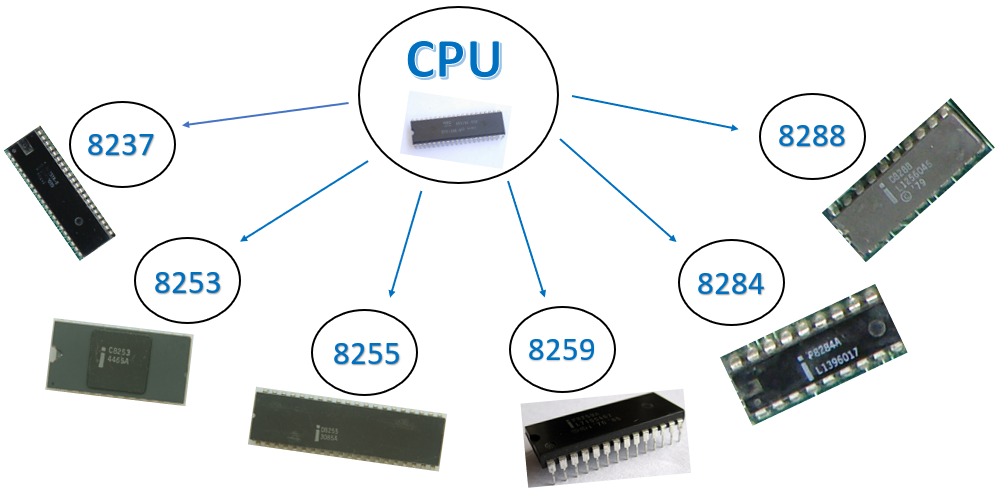
\includegraphics[width=12cm]{images/prech}
		\end{wrapfigure}
		\begin{Large}{
		\vspace{-4cm}Situazione pre-chipset\footnote{Fonte foto: Wikipedia}}
		\end{Large}
	\end{frame}

	\begin{frame}
	\frametitle{\begin{LARGE}Chipset\end{LARGE}}
	Prima del chipset la CPU era collegata a più chip, ognuno dei quali svolgeva delle funzione diverse. 
	\end{frame}

	\begin{frame}
	\frametitle{\begin{LARGE}Chipset\end{LARGE}}
	\begin{wrapfigure}{1}{7cm}
		\vspace{-1.3cm}	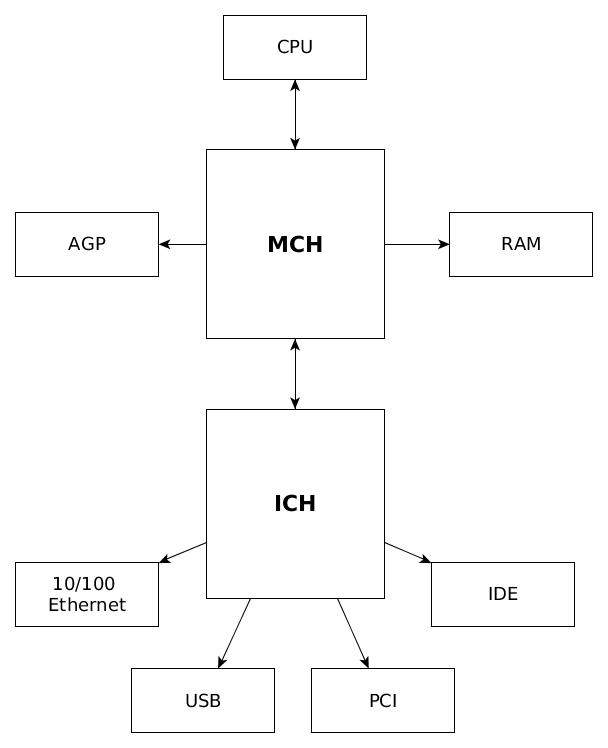
\includegraphics[width=6cm]{images/ciaone}
	\end{wrapfigure}
	\begin{Large}{
			\vspace{-1.5cm}Con l'introduzione \\del chipset viene\\adottato l'\textbf{IHA}\footnote{Fonte foto: Federico Bassignana}\\(Intel Hub\\\vspace{0.2cm} Architecture)}
	\end{Large}
	\end{frame}

	\begin{frame}
	\frametitle{\begin{LARGE}Chipset\end{LARGE}}
	\begin{LARGE}
		\textbf{Intel Hub Architecture}
	\end{LARGE}\par
	\vspace{1cm}
	\begin{Large}
	

	L'Intel Hub Architecture è costituito da due chip principali, l'\textbf{MCH}, Memory Controller Hub e l'\textbf{ICH}, I/O Controller Hub. L'MCH si occupa del controllo e supporto della memoria, mentre l'ICH fornisce connessione per le varie interfacce PCI, USB, IDE, suono e LAN.	\end{Large}
	\end{frame}   
	
	\begin{frame}
	\frametitle{\begin{LARGE}Chipset\end{LARGE}}
	\begin{wrapfigure}{1}{8cm}
		\vspace{-0.9cm}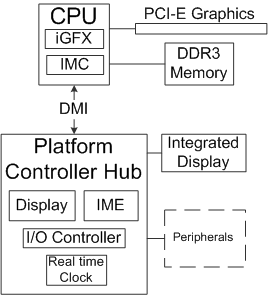
\includegraphics[width=6.5cm]{images/pch}
	\end{wrapfigure}
	\begin{Large}
			\vspace{-3.3cm}
			Successivamente\\ venne utilizzato \\\vspace{0.2cm} il \textbf{PCH}
	\end{Large}
	\end{frame}

	\begin{frame}
	\frametitle{\begin{LARGE}Chipset\end{LARGE}}
	\begin{wrapfigure}{1}{8cm}
		\vspace{-1.3cm}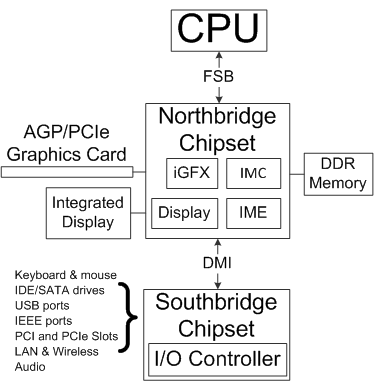
\includegraphics[width=7.8cm]{images/succ}
	\end{wrapfigure}
	\begin{Large}
		\vspace{-2cm}Infine l'organizzazione\\ fu suddivisa \\utilizzando \\\textbf{Northbridge} \\\vspace{0.2cm} e \textbf{Southbidge}
	\end{Large}
	\end{frame}

	\begin{frame}
		\frametitle{\begin{LARGE}Chipset\end{LARGE}}
		\begin{Large}
		\begin{center}
			Chipset example: \textbf{Intel P45} 
		\end{center}	
		\end{Large}
		\begin{itemize}
		\item CPU Support
		\item Memory Support
		\item FSB Frequency
		\item PCIe lanes
		\item Southbridge
		\end{itemize}
	\end{frame}

	\section{Alimentatore}
	\begin{frame}
	\frametitle{\begin{LARGE}Alimentatore - Introduzione\end{LARGE}}
	\begin{wrapfigure}{1}{6cm}
		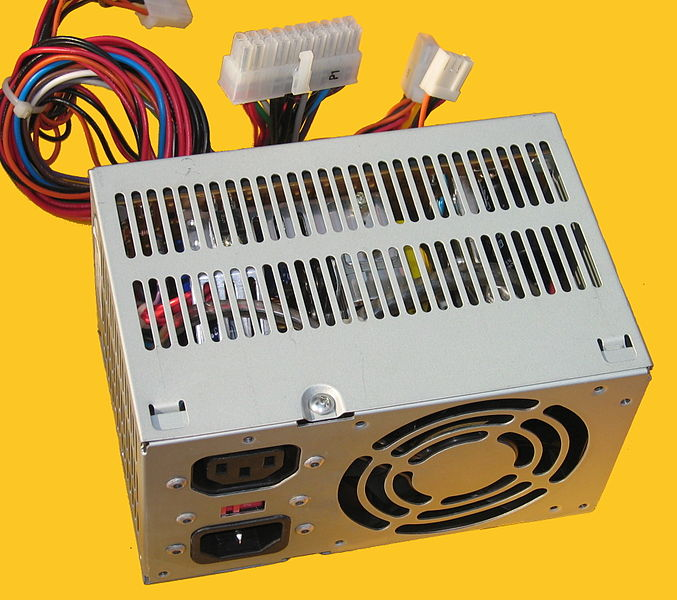
\includegraphics[width=6cm]{images/psu}
	\end{wrapfigure}
	\vspace{-1.5cm}
	\hspace{1cm}
	\begin{Large}
		\hspace{-1cm}\textbf{Vedremo}\par
	\end{Large}
	\begin{itemize}
		\item[-] Connettori di alimentazione
		\item[-] Pinout
		\item[-] Analisi delle tensioni
		\item[-] Funzionamento base alimentatore
	\end{itemize}
	\end{frame}

	\begin{frame}
		\frametitle{\begin{LARGE}Alimentatore\end{LARGE}}
		\begin{wrapfigure}{1}{12cm}
			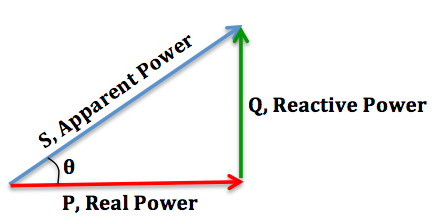
\includegraphics[width=5cm]{images/triang}
		\end{wrapfigure}
		\begin{Large}
			\vspace{-3.5cm}
			\hspace{4.5cm}\textbf{Rendimento}	
		\end{Large}
	\end{frame}

	\begin{frame}
	\frametitle{\begin{LARGE}Alimentatore\end{LARGE}}
	\begin{Large}
		\vspace{-1cm}
		\textbf{Fattori di forma}:
	\end{Large}
	\begin{itemize}
		\item[-] ATX:\par
		\begin{itemize}
			\item TFX
			\item SFX
			\item Flex ATX
			\item Redundant 
		\end{itemize}
		\item[-] Altri
	\end{itemize}

	\end{frame}


\end{document}
